\documentclass[smaller,xcolor=dvipsnames]{beamer}
\usetheme[english]{Berlin}
%\usepackage{ngerman}
\usepackage[ngerman]{babel}
\useoutertheme{infolines}
\beamertemplatenavigationsymbolsempty
\setbeamertemplate{caption}[numbered]
\usepackage{pgfplots,tikz,subfigure}
\usepackage{amsmath,amsthm}
\usepackage{hyperref,graphics,graphicx,color,algorithm,algorithmic,enumerate}
\usepackage{mymacros,wrapfig,relsize}
\usepackage{pict2e}
\usepackage[utf8x]{inputenc}
\usepackage{csquotes}

\newcommand{\ri}{\mathrm{i}}
\newcommand{\T}{\mathsf{T}}
\renewcommand{\H}{\mathsf{H}}
\newcommand{\eps}{\varepsilon}
\newcommand{\To}{\rightarrow}
\newcommand{\sddots}{\scalebox{0.6}{$\ddots$}}
\usepackage[pdf]{pstricks}
\usepackage{sansmathfonts}
\usepackage{eurosym}
\usepackage{ulem}
\renewcommand{\O}{\mathcal{O}}
\DeclareMathOperator{\opt}{OPT}
\DeclareMathOperator{\copt}{Compute-OPT}
\DeclareMathOperator{\icopt}{Iterative-Compute-OPT}
\DeclareMathOperator{\ssum}{Subset-Sum}
\newcommand{\opfind}{\text{Find}}
\newcommand{\opunion}{\text{Union}}
\newcommand{\opmakeunionfind}{\text{MakeUnionFind}}
\newcommand{\component}{\text{Component}}
%\usepackage{arev}
%\renewcommand\familydefault{\sfdefault}

\DeclareMathOperator{\loc}{loc}
\DeclareMathOperator{\rank}{rank}
\DeclareMathOperator{\RE}{Re}
\DeclareMathOperator{\IM}{Im}
\DeclareMathOperator{\In}{In}
\DeclareMathOperator{\im}{im}
\DeclareMathOperator{\Gl}{Gl}
\DeclareMathOperator{\spa}{span}
\DeclareMathOperator{\ext}{{ext}}
\DeclareMathOperator{\ind}{ind}
\DeclareMathOperator{\normalrank}{normalrank}
\DeclareMathOperator{\essup}{ess\,sup}
\DeclareMathOperator{\vect}{vec}

\newcommand{\re}{\mathrm{e}}
\newcommand{\ddt}{\tfrac{\mathrm{d}}{\mathrm{d}t}}
\newcommand{\sys}[4]{\left[\begin{array}{c|c} #1 & #2 \\ \hline #3 & #4 \end{array}\right]}

\renewcommand{\tilde}{\widetilde}
\renewcommand{\hat}{\widehat}


\title[]{Optimierung f\"ur Studierende der Informatik}
\subtitle{-- 13. Vorlesung --}
\author[Matthias Voigt]{\textbf{Matthias Voigt$^{1,2}$}}
\institute[]{
\begin{columns}
%\begin{center}
\column{0.45\textwidth}{\centering {$^1$Universit\"at Hamburg \\ Fachbereich Mathematik \\ Hamburg \\ }}
\column{0.45\textwidth}{\centering {$^2$Technische Universit\"at Berlin \\ Institut f\"ur Mathematik \\ Berlin  \\}}
%\end{center}
\end{columns}
}
\date[]{Universit\"at Hamburg
\begin{columns}
\column{0.45\textwidth}{\centering 
\includegraphics[width = 1.2\textwidth]{uhh-logo.png}\\}
\end{columns}
}

\definecolor{tucgreen}{rgb}{0.0,0.5,0.27}
\definecolor{tucred}{rgb}{0.75,0,0}
\definecolor{tucorange}{rgb}{1.0,.5625,0}
\definecolor{mpired}{HTML}{990000}
\definecolor{mpigreen}{HTML}{5C871D}
\definecolor{mpiblue}{HTML}{006AA9}
\definecolor{mpibg1}{HTML}{5D8B8A}
\definecolor{mpibg2}{HTML}{BFDFDE}
\definecolor{mpibg3}{HTML}{A7C1C0}
\definecolor{mpibg4}{HTML}{7DA9A8}
\definecolor{mpigrey}{rgb}{0.9294,0.9294,0.8784}

\newcommand{\Z}{\mathbb{Z}}

\begin{document}

\maketitle

\begin{frame}
\frametitle{Der Algorithmus von Bellman und Ford}
Es sei $G=(V,E)$ ein gerichteter Graph; jede Kante $e$ von $G$ sei mit einem \alert{Gewicht} $c(e) \in \R$ versehen, wobei auch $c(e) < 0$ gelten kann. \\ \medskip

Mögliche Interpretationen: Die Zahlen $c(e)$ geben \alert{Kosten} an; negative Kosten lassen sich als Einnahmen interpretieren. Statt \enquote{Gewicht} werden wir im Folgenden häufig auch \enquote{Kosten} oder \enquote{Länge} sagen. \\ \medskip

Ist $G'=(V',E')$ ein Teilgraph von $G=(V,E)$, so bezeichnen wir mit $c(G')$ die Summe der Gewichte $c(e)$ für alle Kanten $e$ von $G'$. Es gilt also
\[
c(G') = \sum\limits_{e \in E'}{c(e)}.
\]

\end{frame}

\begin{frame}
\frametitle{Negative Kreise}
 \textbf{Definition:} Ein gerichteter Kreis $C$ von $G$ wird ein \structure{negativer Kreis} genannt, falls $c(C)<0$ gilt. \\ \medskip

Ein negativer Kreis:

\begin{center}
 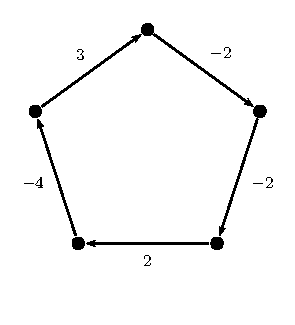
\includegraphics{fig95.pdf}
\end{center}
\end{frame}

\begin{frame}
\frametitle{Zwei eng verwandte Probleme}
\textbf{Zwei eng verwandte Probleme:}
\begin{itemize}
\item \alert{Das Problem der negativen Kreise:} Entscheide, ob $G$ einen negativen Kreis besitzt.
\item \alert{Das Problem der kostenminimalen Pfade:} Gegeben seien ein Graph $G$ ohne negative Kreise sowie ein Knoten $s$ von $G$. Finde für jedes $t$, das von $s$ aus erreichbar ist, einen $s,t$-Pfad $P: s~=~v_0,\ldots,v_k=t$ mit Kanten $e_i=(v_{i-1},v_i)$ ($i=1,\ldots,k$), so dass die Summe
\[
c(P) = \sum\limits_{i=1}^k{c(e_i)}
\]
so klein wie möglich ist.
\end{itemize} \medskip

Statt \enquote{kostenminimaler $s,t$-Pfad} sagen wir auch \structure{kürzester $s,t$-Pfad}.
\end{frame}

\begin{frame}
\frametitle{Kostenminimale Kreise}
 Wir wollen uns zunächst mit dem zweiten Problem, dem Problem der \alert{kostenminimalen Pfade} be\-schäf\-ti\-gen. Der Grund, weshalb in diesem Problem die Existenz negativer Kreise ausgeschlossen wird, liegt auf der Hand:
 \\ \medskip
 
 Andernfalls könnte es vorkommen, dass $t$ zwar von $s$ aus erreichbar ist, es aber trotzdem keinen kürzesten $s,t$-Pfad gibt. Man erkennt dies beispielsweise an der folgenden Darstellung: Zu jeder Zahl $K < 0$ kann man im dargestellten Graphen einen $s,t$-Pfad finden, dessen Länge kleiner als $K$ ist -- man muss den Kreis nur oft genug durchlaufen.

\begin{center}
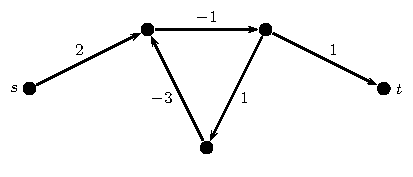
\includegraphics{fig96.pdf}
\end{center}
\end{frame}

\begin{frame}
\frametitle{Eine grundlegende Feststellung}
 Der dynamische Programmierungs-Algorithmus, den wir entwickeln werden, fußt auf der folgenden Feststellung. \\ \medskip

\textbf{Feststellung 1:} Der Graph $G$ besitze keine negativen Kreise und $t$ sei ein von $s$ aus erreichbarer Knoten. \alert{Dann gibt es immer einen kürzesten $s,t$-Pfad, der einfach ist} und demnach höchstens $n-1$ Kanten besitzt\footnotemark. \\ \medskip
\footnotetext{Erklärung: Unter einem \structure{einfachen Pfad} wird hier ein Pfad ohne Knotenwiederholung verstanden. Mit $n$ sei immer die Anzahl der Knoten von $G$ bezeichnet.}
Diese Feststellung ist anschaulich einleuchtend. \\ \medskip

\textbf{Beweisidee:} Bewegt man sich auf einem kürzesten Pfad von $s$ nach $t$, so können nicht-negative Kreise auslassen werden. (Einen formalen Beweis, der auf dieser einfachen Idee beruht, findet man im Skript.)
\end{frame}

\begin{frame}
\frametitle{Definition von $\opt(i,v)$}
 Im Folgenden sei immer ein Knoten $s$ als \enquote{Startpunkt} fest gewählt. Für $v \in V$ und $i \in \bigl\{ 0,1,2,\ldots \bigr\}$ bezeichne $\opt{(i,v)}$ die kleinstmöglichen Kosten $c(P)$ eines $s,v$-Pfades $P$ \alert{mit höchstens $i$ Kanten} -- vorausgesetzt, ein solcher $s,v$-Pfad existiert. \\ \medskip

Falls kein $s,v$-Pfad mit höchstens $i$ Kanten existiert, so setzen wir $\opt{(i,v)}=\infty$. Beispielsweise gilt $\opt{(0,s)}=0$ und $\opt{(0,v)}=\infty$ für alle Knoten $v \neq s$. \\ \medskip

Aufgrund der vorangegangenen Feststellung 1 handelt es sich bei
\[
\opt{(n-1,t)}
\]
um die Größe, die wir berechnen wollen (für alle $t \in V$).
\end{frame}

\begin{frame}
\frametitle{Darstellung von $\opt(i,v)$ durch kleinere Teilprobleme}
 Zunächst geht es aber darum, für $i > 0$ die Größe $\opt{(i,v)}$ mithilfe von kleineren Teilproblemen auf eine möglichst einfache Art auszudrücken. Bislang war dies immer dadurch geschehen, dass wir zwei Fälle unterschieden haben ($n \in \O$ und $n \notin \O$). \\ \medskip
 
 \alert{Diesmal werden wir jedoch wesentlich mehr Fälle unterscheiden}. Wir nehmen an, dass $i > 0$ gilt und stellen uns vor, dass $P$ ein $s,v$-Pfad mit höchstens $i$ Kanten ist, für den $c(P) = \opt{(i,v)}$ gilt. \\ \medskip

Wir unterscheiden die Fälle, dass $P$ höchstens $i-1$ Kanten besitzt und dass $P$ genau $i$ Kanten hat.
\end{frame}

\begin{frame}
\frametitle{Betrachtung von $P$}
 Im ersten Fall ergibt sich Folgendes:
\begin{itemize}
\item \alert{Falls $P$ höchstens $i-1$ Kanten besitzt,} so gilt $\opt{(i,v)} = \opt{(i-1,v)}$.
\end{itemize} \medskip

 Im Fall, dass $P$ genau $i$ Kanten hat, sei der Vorgänger von $v$ auf $P$ mit $u$ bezeichnet (siehe Zeichnung).

\begin{center}
 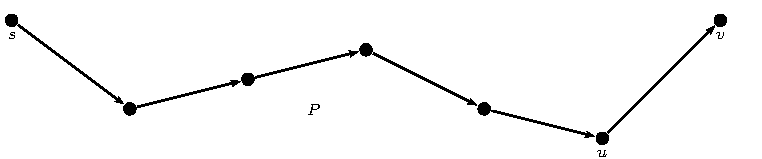
\includegraphics{fig97.pdf}
\end{center}

Es folgt:
\begin{itemize}
\item \alert{Falls $P$ genau $i$ Kanten enthält,} so gilt $\opt{(i,v)} = \opt{(i-1,u)} + c(u,v)$.
\end{itemize}
\end{frame}

\begin{frame}
\frametitle{Die Menge $N^-(v)$}
 \textbf{Bezeichnung:} Ist ein beliebiges $v \in V$ gegeben, so betrachten wir \alert{die Menge aller Knoten $w \in V$, für die die Kante $(w,v)$ in $G$ vorhanden ist.} Da diese Menge im Folgenden eine besondere Rolle spielen wird, führen wir eine Bezeichnung für sie ein:
\[
N^-(v) = \Bigl\{ w \in V : (w,v) \in E \Bigr\}
\] \medskip

Zur Illustration ein \textbf{Beispiel}:
\end{frame}

\begin{frame}
\frametitle{Ein Beispiel}
\begin{center}
 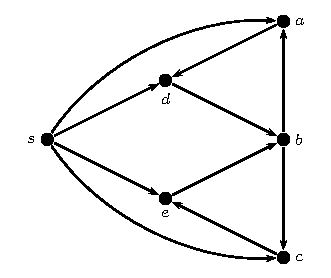
\includegraphics[scale = 1]{fig98.pdf}
\end{center}

Dann gilt:
\begin{align*}
N^-(s) &= \emptyset, \quad\quad\quad N^-(a) = \{ s,b \}, \\
N^-(b) &= \{ d,e \}, \quad N^-(c) = \{ s,b \}, \\
N^-(d) &= \{ s,a \}, \quad N^-(e) = \{ s,c \}.
\end{align*}
\end{frame}

\begin{frame}
\frametitle{Die Rekursionsformel}
 Aus den zuvor gemachten Beobachtungen ergibt sich die folgende \alert{rekursive Formel (f\"ur $i>0$):}
\begin{equation}
\label{eq:13:5}
\opt{(i,v)} = \min \Big\{ \opt{(i-1,v)}, \min\limits_{w \in N^-(v)}\big\{ \opt{(i-1,w)} + c(w,v) \big\}\Big\}.
\end{equation}

Unter Verwendung der Rekursionsformel (\ref{eq:13:5}) erhält man den folgenden dynamischen Pro\-gram\-mie\-rungs-Algorithmus zur Berechnung von $\opt{(n-1,t)}$ für alle $t \in V$, der als \structure{Algorithmus von Bellman und Ford} bekannt ist.
\end{frame}

\begin{frame}
\frametitle{Der Algorithmus von Bellman und Ford}
\begin{center}
\begin{tabular}{rl}
\multicolumn{2}{l}{\textbf{Shortest-Path$(G,c,s)$}} \\
 (1)& $n$ = Anzahl der Knoten in $G$.\\
 (2)& Array $M[0\ldots n-1,V]$. \\
 (3)& Definiere $M[0,s]=0$ und $M[0,v]=\infty$ für alle $v \neq s$. \\
 (4)& \textbf{for} $i=1,\ldots,n-1$ \\ 
 (5)& \qquad \textbf{for} $v \in V$ in beliebiger Reihenfolge \\
 (6)& \qquad\qquad Berechne $M[i,v]$ mittels \eqref{eq:13:5}. \\
 (7)& \qquad \textbf{end for} \\
 (8)& \textbf{end for} \\
 (9)& \textbf{return} $M[n-1,t]$ für alle $t \in V$.
\end{tabular}
\end{center}

Die Korrektheit dieser Methode ergibt sich direkt aus der Rekursion \eqref{eq:13:5} (durch vollständige Induktion). 
\end{frame}

\begin{frame}
\frametitle{Die Laufzeit des Algorithmus von Bellman und Ford}
Für die Laufzeit erhält man Folgendes: \\ \medskip
 
Das Array $M$ hat $n^2$ Einträge und zur Berechnung eines einzelnen Eintrags sind höchstens $n$ Additionen und höchstens $n$ Vergleiche zweier Zahlen erforderlich (vgl. (\ref{eq:13:5})). Insgesamt benötigt der Algorithmus also $O(n^3)$ Operationen, wobei unter einer Operation hier eine Addition oder ein Vergleich zweier Zahlen verstanden werden soll. \\ \medskip

Wir erläutern die Arbeitsweise des Algorithmus von Bellman-Ford anhand des folgenden \textbf{Beispiels}:
\end{frame}

\begin{frame}
\frametitle{Ein Beispiel}
\begin{center}
 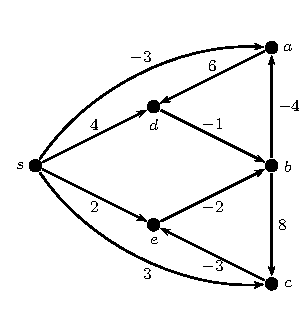
\includegraphics{fig99.pdf}
\end{center}

Das Array $M$ stellen wir als eine $6 \times 6$-Matrix dar, in die anfangs nur die Werte der ersten Zeile eingetragen sind. \alert{Danach werden die Einträge zeilenweise berechnet, wobei sich die Werte der $i$-ten Zeile unter Benutzung von \eqref{eq:13:5} aus der $(i-1)$-ten Zeile ergeben.} Man erhält die folgende Matrix $M$:
\end{frame}

\begin{frame}
\frametitle{Die Matrix $M$}
\begin{center}
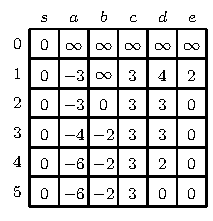
\includegraphics[scale=1.2]{fig100.pdf}
\end{center}
\alert{Für jeden Knoten $t \in V$ lässt sich in der letzten Zeile von $M$ die Länge eines kürzesten $s,t$-Pfades in $G$ ablesen.} Beispielsweise erhält man:
\begin{itemize}
\item die Länge eines kürzesten $s,a$-Pfades ist gleich $-6$;
\item die Länge eines kürzesten $s,d$-Pfades ist gleich $0$.
\end{itemize}

\end{frame}

\begin{frame}
\frametitle{Es lässt sich noch mehr ablesen}
Aufgrund der Konstruktion besitzen auch \alert{die Einträge der übrigen Zeilen eine anschauliche Bedeutung;} beispielsweise bedeutet der Eintrag 2 in der vorletzten Zeile:
\begin{itemize}
\item Die Länge eines kürzesten $s,d$-Pfades mit höchstens vier Kanten ist gleich 2.
\end{itemize} \medskip

Will man nicht nur die Längen kürzester Pfade berechnen, sondern auch entsprechende Pfade $P$ selbst, so ist es zweckmäßig, \alert{zusätzlich zum Wert $\opt{(i,v)}$ einen Knoten $w$ zur Verfügung zu haben, der auf einem entsprechenden Pfad der direkte Vorgänger von $v$ ist} (für $v \neq s$ und falls $\opt{(i,v)} \neq \infty$).

\end{frame}

\begin{frame}
\frametitle{Zusätzliche Berechnung der kürzesten Pfade}
Zu jedem Eintrag $\opt{(i,v)}$, für den $v \neq s$ und $\opt{(i,v)} \neq \infty$ gilt, speichern wir deshalb in $M$ als zusätzliche Information einen Knoten:
\begin{itemize}
\item Falls $\opt{(i,v)}=\opt{(i-1,v)}$ gilt, so sei dies derselbe Knoten, der zuvor zusammen mit $\opt{(i-1,v)}$ gespeichert wurde.
\item Andernfalls speichere man einen Knoten $w \in N^-(v)$, für den gilt:
\[
\opt{(i,v)} = \opt{(i-1,w)} + c(w,v).
\]
\end{itemize} \medskip

\alert{Mithilfe dieser zusätzlichen Einträge lässt sich dann $P$ zurückverfolgen:} Wir schauen uns dies in unserem Beispiel an. Die durch Zusatzeinträge ergänzte Matrix sieht in unserem Beispiel wie folgt aus:
\end{frame}

\begin{frame}
\frametitle{Die erweiterte Matrix}
\begin{center}
 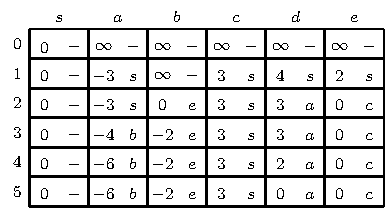
\includegraphics{fig101.pdf}
\end{center}

Wir haben weiter oben bereits festgestellt: Die Länge eines kürzesten $s,d$-Pfades ist gleich $0$. Um zusätzlich einen kürzesten $s,d$-Pfad $P$ zu ermitteln, \alert{benötigen wir nur die letzte Zeile:} Es ergibt sich (Details im Skript):
\[
P = (s,c,e,b,a,d).
\]
\end{frame}

\begin{frame}
\frametitle{Von $s$ aus erreichbare negative Kreise}
 Wir haben bislang vorausgesetzt, dass $G$ keine negativen Kreise enthält. Der Grund dafür war, dass negative Kreise -- sofern sie von $s$ aus erreichbar sind -- für unsere Fragestellung äußerst \enquote{schädlich} sind: vgl. das Beispiel vor Feststellung 1. \\ \medskip

\alert{Wie findet man nun heraus, ob von $s$ aus erreichbare, negative Kreise vorhanden sind?} \\ \medskip

\alert{Zum Glück ist das ganz einfach:} Man hat nichts weiter zu tun, als den Algorithmus von Bellman und Ford wie gewohnt auf $G$ anzuwenden und ganz am Ende noch zusätzlich eine $n$-te Runde einzulegen, d.h., man berechnet durch Anwenden der Formel (\ref{eq:13:5}) zusätzlich Werte $M[n,v]$ für alle $v \in V$; dadurch erhält die Matrix $M$ eine zusätzliche Zeile. Es gilt die folgende Feststellung:
\end{frame}

\begin{frame}
\frametitle{Von $s$ aus erreichbar negative Kreise}
\textbf{Feststellung 2:} $G$ enthält genau dann einen negativen Kreis, der von $s$ aus erreichbar ist, wenn $M[n,v] \neq M[n-1,v]$ für mindestens ein $v \in V$ gilt. \\ \medskip

\textbf{Anders gesagt:}
\begin{itemize}
\item Stimmt die letzte Zeile (d.h. die Zeile mit den Werten $M[n,v]$) \textbf{nicht} mit der vorletzten Zeile überein, \alert{so brechen wir das Verfahren ab} mit dem Ergebnis, dass ein von $s$ aus erreichbarer negativer Kreis vorhanden ist.

\item Stimmen die beiden genannten Zeilen dagegen überein, so gibt es keine von $s$ aus erreichbaren negativen Kreise in $G$. \alert{In diesem Fall können wir die Länge kürzester $s,t$-Pfade an der letzten (oder vorletzten) Zeile von $M$ ablesen;} dabei bedeutet der Eintrag $\infty$, dass der entsprechende Knoten nicht von $s$ erreichbar ist.
\end{itemize}
\end{frame}

\begin{frame}
\frametitle{Kürzeste Pfade \enquote{all-to-all}: Der Algorithmus von Floyd und Warshall}
 Gegeben sei ein gerichteter Graph $G=(V,E)$. Die Knoten von $G$ seien mit $1,\ldots,n$ bezeichnet, es gelte also $V = \{ 1,\ldots,n \}$. Außerdem sei für jede gerichtete Kante $(i,j) \in E$ ein Gewicht $w_{ij}$ gegeben, wobei $w_{ij} < 0$ erlaubt ist. Mit $w$ sei die Abbildung bezeichnet, die jeder Kante von $G$ ihr Gewicht $w_{ij}$ zugeordnet. Unter den genannten Voraussetzungen sprechen wir auch von einem \structure{gewichteten Graphen} $(G,w)$. \\ \medskip

Ist nichts anderes gesagt, so seien negative Kreise ausgeschlossen. Statt vom \enquote{Gewicht} einer Kante sprechen wir auch von ihrer \structure{Länge} oder ihren \structure{Kosten}. Unter dem \structure{Abstand} (oder der \structure{Distanz}) von $i$ nach $j$ verstehen wir die Länge eines kürzesten $i,j$-Pfades in $G$.
\end{frame}

\begin{frame}
\frametitle{All-to-All}
 In manchen Situationen möchte man nicht nur die Abstände von einem festen Knoten $s$ berechnen (\enquote{one-to-all}), sondern man interessiert sich für die \alert{Abstände zwischen sämtlichen Knotenpaaren} (\enquote{all-to-all}). \\ \medskip

Eine Möglichkeit, das Problem \enquote{all-to-all} zu behandeln, besteht darin, den Algorithmus von Bellman und Ford wiederholt anzuwenden, wobei jeder der $n$ Knoten genau einmal die Rolle des Ausgangsknotens $s$ übernimmt. Da der Algorithmus von Bellman und Ford  die Komplexität $O(n^3)$ besitzt, gelangt man auf diese Art zu einem Algorithmus der Komplexität \alert{$O(n^4)$.}
\end{frame}

\begin{frame}
\frametitle{Komplexität des Algorithmus von Floyd und Warshall}
Der häufig benutzte \structure{Algorithmus von Floyd und Warshall}, den wir im Folgenden besprechen werden, löst ebenfalls das Problem \enquote{all-to-all}; er ist jedoch effizienter als die zuvor beschriebene Methode: \alert{Die Komplexität des Algorithmus von Floyd und Warshall ist $O(n^3)$.} \\ \medskip

Für $i \neq j$ setzen wir zusätzlich $w_{ij} = \infty$, falls es in $G$ keine von $i$ nach $j$ gerichtete Kante gibt. \\ \medskip

Der Algorithmus von Floyd und Warshall ist sehr einfach zu beschreiben und auszuführen. Wir legen hier die Darstellung aus dem Buch von Jungnickel zugrunde (mit leichten Modifikationen):
\end{frame}

\begin{frame}
\frametitle{Algorithmus von Floyd und Warshall}
\begin{center}
\begin{tabular}{rl}
%\multicolumn{2}{l}{\textbf{Algorithmus von Floyd und Warshall}} \\
 (1)& \textbf{for } $i=1$ \textbf{ to } $n$ \textbf{ do} \\
 (2)& \qquad \textbf{for } $j=1$ \textbf{ to } $n$ \textbf{ do} \\
 (3)& \qquad\qquad \textbf{if } $i \neq j$ \textbf{ then } \\
 (4)& \qquad\qquad \qquad $d(i,j) \leftarrow w_{ij}$ \\
 (5)& \qquad\qquad \textbf{ else } \\
 (6)& \qquad\qquad\qquad $d(i,j) \leftarrow 0$ \\ 
 (7)& \qquad\qquad \textbf{end if} \\
 (8)& \qquad \textbf{end do} \\
 (9)& \textbf{end do} \\
 (10)& \textbf{for } $k=1$ \textbf{ to } $n$ \textbf{ do} \\
 (11)& \qquad \textbf{for } $i=1$ \textbf{ to } $n$ \textbf{ do} \\
 (12)& \qquad\qquad \textbf{for } $j=1$ \textbf{ to } $n$ \textbf{ do} \\
 (13)& \qquad\qquad\qquad \textbf{if } $i \neq k$ \textbf{ and } $j \neq k$ \textbf{ then } \\
 (14)& \qquad\qquad\qquad\qquad $d(i,j) \leftarrow \min\bigl\{ d(i,j), d(i,k) + d(k,j) \bigr\}$ \\
(15)& \qquad\qquad\qquad \textbf{end if} \\
(16)& \qquad\qquad \textbf{end do} \\
(17)& \qquad \textbf{end do} \\
(18)& \textbf{end do} \\
\end{tabular}
\end{center}
\end{frame}

\begin{frame}
\frametitle{Die Matrizen $D_0,\ldots,D_n$}
 Mit $D_0 = \left( d_{ij}^{(0)} \right)$ sei die $n \times n$ - Matrix bezeichnet, die durch die Zeilen (3)--(7) definiert wird. \\ \medskip
 
 Außerdem: $D_k = \left( d_{ij}^{(k)} \right)$ sei die Matrix, die im $k$-ten Durchlauf der äußeren For-Schleife (Zeile (10)--(18)) generiert wird ($k=1,\ldots,n$). \\ \medskip

Für alle $k \in \bigl\{ 0,\ldots,n \bigr\}$ und alle $i,j \in \bigl\{ 1,\ldots,n \bigr\}$ bezeichnen wir mit
\[
\mathcal{P}_{ij}^{(k)}
\]
die Menge aller $i,j$-Pfade $P$ von $G$, für die gilt:
\begin{equation}
\tag{$\star$}
\alert{\text{Es gibt in $P$ keine inneren Knoten $\ell$, für die $\ell > k$ gilt.}}
\end{equation}
\end{frame}

\begin{frame}
\frametitle{Innere Knoten}
 Etwas anders gesagt: $P \in \mathcal{P}_{ij}^{(k)}$ bedeutet, dass $P$ ein $i,j$-Pfad ist, bei dem Knoten $\ell$ mit $\ell > k$ als innere Knoten nicht vorkommen (siehe Skizze).

\begin{center}
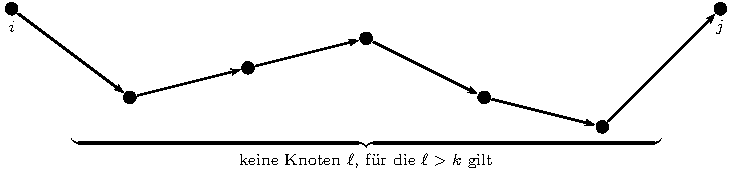
\includegraphics{fig102.pdf}
\end{center}

In der nachfolgenden Feststellung, die man unschwer durch vollständige Induktion beweist (als Übungsaufgabe empfohlen!), wird die Bedeutung der Einträge $d_{ij}^{(k)}$ der Matrizen $D_k$ festgehalten.
\end{frame}

\begin{frame}
\frametitle{Interpretation von $d_{ij}^{(k)}$}
\textbf{Feststellung:}
Für alle $k=0,1,\ldots,n$ sowie für alle $i,j \in \{ 1,\ldots,n \}$ gilt:
\begin{itemize}
\item Falls $\mathcal{P}_{ij}^{(k)} \neq \emptyset$, so gibt $d_{ij}^{(k)}$ die kleinstmögliche Länge eines Pfades $P \in \mathcal{P}_{ij}^{(k)}$ an.
\item Falls $\mathcal{P}_{ij}^{(k)} = \emptyset$, so gilt $d_{ij}^{(k)} = \infty$.
\end{itemize} \medskip

Da $D_n = \left( d_{ij}^{(n)} \right)$ die Matrix ist, die der Algorithmus von Floyd und Warshall am Ende abliefert, interessiert uns natürlich der Fall $k=n$ ganz besonders. Schaut man sich die Bedingung ($\star$) für den Fall $k=n$ an, so erkennt man, dass es sich bei
\[
\mathcal{P}_{ij}^{(n)}
\]
um die Menge \alert{sämtlicher} $i,j$-Pfade in $G$ handelt. 
\end{frame}

\begin{frame}
\frametitle{Ein Beispiel}
Für den Fall $k=n$ bedeutet unsere Feststellung also:
 \begin{itemize}
\item \alert{Falls es in $G$ einen $i,j$-Pfad gibt, so gibt $d_{ij}^{(n)}$ die Länge eines kürzesten $i,j$-Pfades in $G$ an.}
\item \alert{Falls es in $G$ keinen $i,j$-Pfad gibt, so gilt $d_{ij}^{(n)} = \infty$.}
\end{itemize}

\textbf{Beispiel:} Wir betrachten den folgenden Graphen mit Kantengewichten $w_{ij}$ wie angegeben:

\begin{center}
 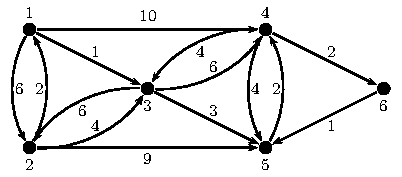
\includegraphics{fig103.pdf}
\end{center}
\end{frame}

\begin{frame}
\frametitle{Die Matrix $D_0$}
 Man erhält die folgende Matrix $D_0$:
\[
D_0 =
\begin{bmatrix}
0 & 6 & 1 & 10 & \infty & \infty \\
2 & 0 & 4 & \infty & 9 & \infty \\
\infty & 6 & 0 & 6 & 3 & \infty \\
\infty & \infty & 4 & 0 & 4 & 2 \\
\infty & \infty & \infty & 2 & 0 & \infty \\
\infty & \infty & \infty & \infty & 1 & 0
\end{bmatrix}.
\] \medskip

\alert{Es gibt im Folgenden keine Veranlassung mehr, auf die Zeichnung zu schauen:} Die gesamte Information der Zeichnung wurde in die Matrix $D_0$ übertragen.
\end{frame}

\begin{frame}
\frametitle{Übergang von $D_{k-1}$ zu $D_k$}
 Die Matrix $D_k$ erhält man aus der Matrix $D_{k-1}$, indem man die folgenden Rekursionsformeln anwendet:

Für $k = 1,\ldots,n$ gilt:
\begin{align}
\label{eq:13:6}
d_{ij}^{(k)} &= d_{ij}^{(k-1)} \text{ falls } i=k \text{ oder } j=k \\
\label{eq:13:7}
d_{ij}^{(k)} &= \min\Bigl\{ d_{ij}^{(k-1)}, d_{ik}^{(k-1)} + d_{kj}^{(k-1)} \Bigr\} \text{ falls } i \neq k \text{ und } j \neq k.
\end{align} \medskip

Man mache sich klar, dass sich die Formeln \eqref{eq:13:6} und \eqref{eq:13:7} unmittelbar aus den Zeilen (13)--(15) des Algorithmus von Floyd und Warshall ergeben. \\ \medskip

\alert{Aufgrund von \eqref{eq:13:6} ändern sich beim Übergang von $D_{k-1}$ zu $D_k$ die $k$-te Zeile und die $k$-te Spalte nicht.} Führt man den Algorithmus von Floyd und Warshall per Hand aus, so ist es beim Aufstellen der Matrix $D_k$ zweckmäßig, zunächst die $k$-te Zeile und die $k$-te Spalte von $D_{k-1}$ direkt in $D_k$ zu übernehmen.
\end{frame}

\begin{frame}
\frametitle{Der Übergang von $D_0$ nach $D_1$}
 Gehen wir in unserem Beispiel von $D_0$ zu $D_1$ über, so schreiben wir also zunächst die 1. Zeile und die 1. Spalte von $D_0$ ab; man erhält eine Matrix, in der die meisten Einträge noch fehlen:
\[
\begin{bmatrix}
0 & 6 & 1 & 10 & \infty & \infty \\
2 & \cdot & \cdot & \cdot & \cdot & \cdot \\
\infty & \cdot & \cdot & \cdot & \cdot & \cdot \\
\infty & \cdot & \cdot & \cdot & \cdot & \cdot \\
\infty & \cdot & \cdot & \cdot & \cdot & \cdot \\
\infty & \cdot & \cdot & \cdot & \cdot & \cdot
\end{bmatrix}.
\]

Danach trägt man dann gemäß \eqref{eq:13:7} die übrigen Einträge ein; man erhält
\[
D_1 = 
\begin{bmatrix}
\color{Green}{0} & \color{Green}{6} & \color{Green}{1} & \color{Green}{10} & \color{Green}{\infty} & \color{Green}{\infty} \\
\color{Green}{2} & 0 & 3 & 12 & 9 & \infty \\
\color{Green}{\infty} & 6 & 0 & 6 & 3 & \infty \\
\color{Green}{\infty} & \infty & 4 & 0 & 4 & 2 \\
\color{Green}{\infty} & \infty & \infty & 2 & 0 & \infty \\
\color{Green}{\infty} & \infty & \infty & \infty & 1 & 0
\end{bmatrix}.
\]
\end{frame}

\begin{frame}
\frametitle{Entstehung von $D_2$}
In ähnlicher Weise erhält man $D_2$, indem man zunächst die 2. Zeile und die 2. Spalte von $D_1$ abschreibt:
\[
\begin{bmatrix}
\cdot & 6 & \cdot & \cdot & \cdot & \cdot \\
2 & 0 & 3 & 12 & 9 & \infty \\
\cdot & 6 & \cdot & \cdot & \cdot & \cdot \\
\cdot & \infty & \cdot & \cdot & \cdot & \cdot \\
\cdot & \infty & \cdot & \cdot & \cdot & \cdot \\
\cdot & \infty & \cdot & \cdot & \cdot & \cdot
\end{bmatrix}.
\]

Anschließendes Auffüllen der Matrix gemäß \eqref{eq:13:7} ergibt
\[
D_2 =
\begin{bmatrix}
0 & \color{Green}{6} & 1 & 10 & 15 & \infty \\
\color{Green}{2} & \color{Green}{0} & \color{Green}{3} & \color{Green}{12} & \color{Green}{9} & \color{Green}{\infty} \\
8 & \color{Green}{6} & 0 & 6 & 3 & \infty \\
\infty & \color{Green}{\infty} & 4 & 0 & 4 & 2 \\
\infty & \color{Green}{\infty} & \infty & 2 & 0 & \infty \\
\infty & \color{Green}{\infty} & \infty & \infty & 1 & 0
\end{bmatrix}.
\]
\end{frame}

\begin{frame}
\frametitle{$D_3$ und $D_4$}
Fährt man entsprechend fort, so erhält man der Reihe nach die folgenden Matrizen (Prüfen Sie dies nach!):
\[
D_3 =
\begin{bmatrix}
0 & 6 & \color{Green}{1} & 7 & 4 & \infty \\
2 & 0 & \color{Green}{3} & 9 & 6 & \infty \\
\color{Green}{8} & \color{Green}{6} & \color{Green}{0} & \color{Green}{6} & \color{Green}{3} & \color{Green}{\infty} \\
12 & 10 & \color{Green}{4} & 0 & 4 & 2 \\
\infty & \infty & \color{Green}{\infty} & 2 & 0 & \infty\\
\infty & \infty & \color{Green}{\infty} & \infty & 1 & 0
\end{bmatrix}.
\]

\[
D_4 =
\begin{bmatrix}
0 & 6 & 1 & \color{Green}{7} & 4 & 9 \\
2 & 0 & 3 & \color{Green}{9} & 6 & 11 \\
8 & 6 & 0 & \color{Green}{6} & 3 & 8 \\
\color{Green}{12} & \color{Green}{10} & \color{Green}{4} & \color{Green}{0} & \color{Green}{4} & \color{Green}{2} \\
14 & 12 & 6 & \color{Green}{2} & 0 & 4 \\
\infty & \infty & \infty & \color{Green}{\infty} & 1 & 0
\end{bmatrix}.
\]
\end{frame}

\begin{frame}
\frametitle{$D_5$ und $D_6$}
\[
D_5 =
\begin{bmatrix}
0 & 6 & 1 & 6 & \color{Green}{4} & 8 \\
2 & 0 & 3 & 8 & \color{Green}{6} & 10 \\
8 & 6 & 0 & 5 & \color{Green}{3} & 7 \\
12 & 10 & 4 & 0 & \color{Green}{4} & 2 \\
\color{Green}{14} & \color{Green}{12} & \color{Green}{6} & \color{Green}{2} & \color{Green}{0} & \color{Green}{4} \\
15 & 13 & 7 & 3 & \color{Green}{1} & 0
\end{bmatrix}.
\]

\[
D_6 =
\begin{bmatrix}
0 & 6 & 1 & 6 & 4 & \color{Green}{8} \\
2 & 0 & 3 & 8 & 6 & \color{Green}{10} \\
8 & 6 & 0 & 5 & 3 & \color{Green}{7} \\
12 & 10 & 4 & 0 & 3 & \color{Green}{2} \\
14 & 12 & 6 & 2 & 0 & \color{Green}{4} \\
\color{Green}{15} & \color{Green}{13} & \color{Green}{7} & \color{Green}{3} & \color{Green}{1} & \color{Green}{0}
\end{bmatrix}.
\] 
\end{frame}

\begin{frame}
\frametitle{Adjazenzmatrix und Distanzmatrix}
 Die Matrix $D_6$ des Beispiels -- bzw. allgemein die vom Algorithmus von Floyd und Warshall gelieferte Matrix $D_n$ -- nennt man die \structure{Distanzmatrix} des gewichteten Graphen $(G,w)$. \\ \medskip
 
 Es ist üblich, auch der Matrix $D_0$ einen Namen zu geben: Man nennt $D_0$ die \structure{Adjazenzmatrix} von $(G,w)$. \\ \medskip
 
 Der Algorithmus von Floyd und Warshall wandelt also die Adjazenzmatrix $D_0$ in die Distanzmatrix $D_n$ um. Dies geschieht stufenweise: Den Matrizen $D_1, \ldots, D_{n-1}$ kommt die Rolle von Zwischenstufen zu. Man beachte, dass für diesen Umwandlungsprozess nur ein einziges $n \times n$ - Array zum Speichern der Matrizeneinträge benötigt wird (vgl. Zeile (14) des Algorithmus).
\end{frame}

\begin{frame}
\frametitle{Komplexität}
 Die Komplexität $O(n^3)$ des Algorithmus von Floyd und Warshall ergibt sich unmittelbar aus den Zeilen (10)--(18). \\ \medskip

In Vorlesung 12 haben wir dargelegt, unter welchen Bedingungen man von einer algorithmischen Lösung mittels \alert{dynamischer Programmierung} spricht. \\ \medskip 

\textbf{Aufgabe:} Überlegen Sie sich, dass der Algorithmus von Floyd und Warshall den in Vorlesung 12 genannten Anforderungen genügt. \\ \medskip

Der Algorithmus von Floyd und Warshall ist also ein weiteres Beispiel für einen Algorithmus der Gattung \alert{\enquote{Dynamische Programmierung}.}
\end{frame}

\begin{frame}
\frametitle{Erweiterungen}
\textbf{Weitere Aufgaben:}
 \begin{enumerate}[1.]
\item Es sei $(G,w)$ ein gewichteter Graph, von dem nicht bekannt ist, ob er einen \alert{negativen Kreis} enthält. Wie kann der Algorithmus von Floyd und Warshall eingesetzt werden, um herauszufinden, ob ein negativer Kreis in $(G,w)$ vorhanden ist?

\item Es ist möglich, den Algorithmus von Floyd und Warshall so zu modifizieren, dass nicht nur die Distanzen für alle Knotenpaare, sondern auch die dazugehörigen kürzesten Pfade geliefert werden. Wie kann das geschehen?
\end{enumerate}
\end{frame}

\begin{frame}
\frametitle{Die Union-Find-Datenstruktur}
Wir gehen auch in diesem Abschnitt nach Kleinberg und Tardos vor. \\ \medskip 

Gegeben sei eine endliche Knotenmenge. Wir befassen uns mit dem Vorgang, dass aus dieser Knotenmenge ein Graph dadurch \enquote{heranwächst}, dass Kanten schrittweise hinzugenommen werden (pro Schritt niemals mehr als eine Kante). \\ \medskip

Am Anfang besteht der Graph nur aus isolierten Knoten, von denen jeder für sich eine Zusammenhangskomponente darstellt. Im Laufe des Verfahrens können Zusammenhangskomponenten zu größeren Komponenten zusammenwachsen.
\end{frame}

\begin{frame}
\frametitle{Die Union-Find-Datenstruktur}
 Wenn eine Kante hinzugefügt wird, so wollen wir die Komponenten natürlich nicht jedes Mal völlig neu berechnen; stattdessen soll eine Datenstruktur zum Einsatz kommen, die ein schnelles Update der Komponenten unterstützt. Außerdem soll diese Datenstruktur erlauben, zu einem gegebenen Knoten $u$ den Namen der Komponente, der $u$ angehört, schnell zu ermitteln. Man spricht von einer \structure{Union-Find-Datenstruktur}. \\ \medskip

 \alert{Um den Algorithmus von Kruskal effizient zu implementieren, benötigt man eine Datenstruktur, die das Beschriebene leistet.}
\end{frame}

\begin{frame}
\frametitle{Anwendung auf den Algorithmus von Kruskal}
Wird im Algorithmus von Kruskal für eine Kante $e=\{u,v\}$ gefragt, ob durch die Hinzunahme von $e$ zum aktuellen Graphen ein Kreis entsteht, so kommt es darauf an, die aktuellen Komponenten von $u$ und $v$ zu bestimmen; man fragt dann, \alert{ob diese Komponenten gleich sind:}
\begin{itemize}
\item Falls ja, so wird $e$ zurückgewiesen, da sonst ein Kreis entstünde.
\item Falls nein, so wird $e$ zum aktuellen Graphen hinzugefügt, wodurch kein Kreis entsteht. Anschließend hat man ein Update der Komponenten vorzunehmen (\enquote{Zusammenlegung der Komponenten von $u$ und $v$}).
\end{itemize}

Union-Find-Datenstrukturen spielen nicht nur im Zusammenhang mit Kruskals Algorithmus eine wichtige Rolle, sondern ebenso im Zusammenhang mit anderen Fragestellungen, bei denen \alert{Partitionen} von Mengen zu verwalten sind. %Aus diesem Grund behandeln wir das Problem, eine geeignete Union-Find-Datenstruktur zu entwickeln, ab jetzt unabhängig von Kruskals Algorithmus und kommen nur gelegentlich darauf zurück.
\end{frame}

\begin{frame}
\frametitle{Die Operationen Find($u$) und Union($A,B$)}
 Wir beschreiben noch einmal, worum es beim Union-Find-Problem geht. \alert{Die zu entwickelnde Union-Find-Datenstruktur soll es ermöglichen, disjunkte Mengen (wie beispielsweise die Knotenmengen der Komponenten eines Graphen) zu verwalten, womit Folgendes gemeint ist}:
\begin{itemize}
\item Für jeden Knoten\footnote{Die Elemente der betrachteten Mengen bezeichnen wir auch dann als Knoten, wenn keine Graphen im Spiel sind.} $u$ soll die \structure{Operation Find($u$)} den Namen der Menge liefern, die $u$ enthält. Die Operation $\opfind(u)$ kann benutzt werden, um zu testen, ob $u$ und $v$ derselben Menge angehören: Man muss lediglich prüfen, ob $\opfind{(u)} = \opfind{(v)}$ gilt.

\item Neben der Operation $\opfind{(u)}$ soll es eine \structure{Operation Union($A,B$)} geben, durch die die beiden Mengen $A$ und $B$ zu einer einzigen Menge vereinigt werden.
\end{itemize}
\end{frame}

\begin{frame}
\frametitle{Die Operation $\opmakeunionfind(A,B)$ und Überblick}
 Neben den Operationen $\opunion{(A,B)}$ und $\opfind{(u)}$ spielt außerdem die \alert{Operation MakeUnionFind($S$)} eine Rolle. Die Operation MakeUnionFind($S$) dient der Initialisierung. Zusammenfassend halten wir fest, dass die Union-Find-Datenstruktur drei Operationen unterstützen soll:
\begin{itemize}
\item Für eine Menge $S$ soll \alert{MakeUnionFind($S$)} eine Partition von $S$ in disjunkte Klassen\footnote{Statt Partition sagt man bekanntlich auch \structure{Zerlegung} und spricht von \structure{Klassen} der Partition (bzw. Zerlegung).} liefern, die alle nur aus einem einzigen Element bestehen. $\opmakeunionfind{(S)}$ wird in $O(n)$ Zeit implementiert werden (für $n = |S|$).

\item Für ein $u \in S$ soll \alert{Find($u$)} den Namen der Klasse liefern, die $u$ enthält. Unser Ziel ist, $\opfind{(u)}$ so zu implementieren, dass $\opfind{(u)}$ nur $O(\log{n})$ Zeit benötigt. (In einigen der vorgestellten Implementierungen wird $\opfind{(u)}$ sogar nur $O(1)$ Zeit in Anspruch nehmen.)

\item Durch \alert{Union($A$,$B$)} sollen zwei Klassen $A$ und $B$ vereinigt werden. Unser Ziel wird sein, die Operation $\opunion{(A,B)}$ so zu implementieren, dass sie nur $O(\log{n})$ Zeit in Anspruch nimmt.
\end{itemize}
\end{frame}

\begin{frame}
\frametitle{Konsistente Namensgebung}
Eine Bemerkung dazu, was unter dem \alert{Namen einer Klasse} zu verstehen ist: Das Wichtigste in diesem Zusammenhang ist, dass die Namensgebung \alert{konsistent} ist, d.h., dass $\opfind{(v)}$ und $\opfind{(w)}$ denselben Namen liefern, wenn $v$ und $w$ aus derselben Klasse stammen und außerdem muss natürlich auch $\opfind{(v)} \neq \opfind{(w)}$ gelten, wenn dies nicht der Fall ist. Darüber hinaus hat man große Freiheiten bei der Namenswahl. \\ \medskip
\alert{Im Folgenden wird immer die naheliegende Lösung gewählt werden, dass eine Klasse nach einem ihrer Elemente benannt wird.}
\end{frame}

\begin{frame}
\frametitle{Union-Find mittels eines Arrays}
 Eine einfache Art, eine Union-Find-Datenstruktur einzurichten, ist mittels eines Arrays, in dem für jedes Element der Name der zugehörigen Klasse angegeben wird. \\ \medskip
 
 \textbf{Genauer:} Es sei $S$ die betrachtete Menge, es gelte $|S|=n$ und die Elemente von $S$ seien mit $1,\ldots,n$ bezeichnet. Es sei \structure{$\component$} ein Array der Länge $n$, wobei $\component[s]$ der Name der Klasse sei, der $s$ angehört ($s=1,\ldots,n$). \\ \medskip
 
 Zur Durchführung von $\opmakeunionfind{(S)}$ wird $\component[s]=s$ gesetzt ($s=1,\ldots,n$); dies bedeutet, dass am Anfang jedes Element $s$ seine eigene individuelle Klasse bildet. $\opmakeunionfind{(S)}$ ist klarerweise in $O(n)$ Zeit durchführbar.
\end{frame}

\begin{frame}
\frametitle{$\opfind(u)$ wird begünstigt}
 Die Implementierung einer Union-Find-Datenstruktur mittels eines Arrays führt dazu, dass die Durch\-füh\-rung von $\opfind{(u)}$ sehr einfach ist: \alert{$\opfind{(u)}$ ist in $O(1)$ Zeit durchführbar, da nichts weiter zu tun ist, als den aktuellen Wert von Component$[u]$ abzulesen}. \\ \medskip

\alert{Im Gegensatz dazu kann die Operation $\opunion{(A,B)}$ jedoch einen Zeitaufwand von $O(n)$ erfordern}, da im Fall $A \neq B$ für eine der beiden Mengen $A$, $B$ sämtliche Einträge $\component[s]$ abzuändern sind. (Man beachte: Beide Mengen $A$ und $B$ können einen konstanten Anteil von $S$ ausmachen, etwa $|A| = \frac{1}{3}n$ und $|B| = \frac{1}{4}n$.)
\end{frame}

\begin{frame}
\frametitle{Zwei nützliche Maßnahmen}
Wir betrachten \alert{zwei Maßnahmen}, um die Operation $\opunion{(A,B)}$ zu verbessern:
\begin{itemize}
\item Es ist nützlich, für jede Klasse zusätzlich eine Liste ihrer Elemente zu führen; dadurch erreicht man, dass nicht jedes Mal das gesamte Array durchgegangen werden muss, wenn für die Elemente einer Klasse ein Update durchzuführen ist.
\item Darüber hinaus spart man einige Zeit, wenn als Name für die durch Zusammenlegung entstandene Klasse der Name von $A$ oder von $B$ übernommen wird. Das hat den Vorteil, dass nur für die Elemente von einer der beiden Klassen ein Update vorgenommen werden muss. Dabei gilt aus naheliegenden Gründen die folgende \alert{Regel}:

\begin{center}
\alert{Falls $A$ und $B$ unterschiedliche Größe haben, so übernimmt man den Namen der größeren Klasse.}
\end{center}
\end{itemize}
\end{frame}

\begin{frame}
\frametitle{Ein zusätzliches Detail}
 Um festzustellen, welche der beiden Klassen die größere ist, kann ein zusätzliches Array \structure{Size} der Länge $n$ verwendet werden, in dem für jedes $s$, das aktuell als Name einer Klasse auftritt, die Größe Size$[s]$ dieser Klasse abgelesen werden kann; hierzu sind pro Union-Operation zwei Einträge des Arrays Size abzuändern.
\end{frame}

\begin{frame}
\frametitle{Schlechte Fälle}
 Auch mit diesen beiden Verbesserungen bleibt es \alert{im schlechtesten Fall} bei einem Zeitaufwand der Größenordnung $O(n)$ für die Union-Operation: \\ \medskip
 
 Dieser Fall tritt ein, wenn es sich bei beiden Mengen $A$ und $B$ um große Mengen handelt, was heißen soll, dass sowohl $A$ als auch $B$ einen konstanten Anteil der Elemente von $S$ umfasst. \alert{Solche schlechten Fälle für $\opunion{(A,B)}$ können allerdings nicht allzu häufig auftreten, da es sich bei $A \cup B$ um eine noch größere Menge handelt}. \\ \medskip
 
 Diese wichtige, aber noch etwas vage Feststellung soll im Folgenden präzisiert werden. Dies geschieht dadurch, dass wir uns weniger die Laufzeit einer einzelnen Operation $\opunion{(A,B)}$ anschauen, sondern die Folge der ersten $k$ Union-Operationen unter die Lupe nehmen, wobei es um die \alert{Gesamtlaufzeit} (bzw. die \alert{durchschnittliche Laufzeit}) dieser $k$ Operationen geht.
\end{frame}

\begin{frame}
\frametitle{Zeitaufwand für die Folge der ersten $k$ Union-Operationen}
\textbf{Satz 1:}
Betrachtet werde die \alert{Array-Implementierung der Union-Find-Datenstruktur}\index{Array-Implementierung der Union-Find-Datenstruktur}\index{Union-Find-Datenstruktur!Array-Implementierung} für eine Menge $S$ mit $|S|=n$, wobei Vereinigungen den Namen der größeren Menge übernehmen sollen. Eine $\opfind$-Operation benötigt dann $O(1)$ Zeit, $\opmakeunionfind{(S)}$ erfordert $O(n)$ Zeit und für die Folge der ersten $k$ $\opunion$-Operationen wird insgesamt höchstens $O(k \log{k})$ Zeit benötigt (für alle $k$, die kleiner oder gleich der Gesamtzahl der Union-Operationen sind). \\ \medskip

\textbf{Beweis:} Die Behauptungen über die $\opfind$-Operation und über $\opmakeunionfind{(S)}$ sind leicht einzusehen. Es geht also um die letzte Behauptung, zu deren Beweis wir die ersten $k$ $\opunion$-Operationen betrachten. 
\end{frame}

\begin{frame}
\frametitle{Zeitaufwand für die Folge der ersten $k$ Union-Operationen}
Der einzige Teil einer $\opunion$-Operation, der mehr als $O(1)$ Zeit in Anspruch nimmt, ist das Update des Arrays $\component$. \alert{Wir betrachten ein festes $v \in S$ und fragen uns, wie oft $\component[v]$ bei der Durchführung unserer $k$ Union-Operationen höchstens geändert werden kann.} \\ \medskip 

 Es sei daran erinnert, dass am Anfang, nachdem $\opmakeunionfind{(S)}$ ausgeführt wurde, alle $n$ Elemente von $S$ eine eigene Klasse bilden. Eine einzige $\opunion$-Operation kann immer nur für höchstens zwei dieser 1-elementigen Klassen bewirken, dass sie zu einer 2-elementigen Klasse verschmelzen. Dies bedeutet, dass nach $k$ $\opunion$-Operationen alle bis auf höchstens $2k$ Elemente von $S$ noch völlig unberührt sind und immer noch lauter 1-elementige Klassen bilden.
\end{frame}

\begin{frame}
\frametitle{Zeitaufwand für die Folge der ersten $k$ Union-Operationen}
 Wir betrachten ein festes Element $v$ aus $S$. Sobald die Klasse von $v$ in eine unserer $k$ $\opunion$-Operationen involviert ist, wächst sie an. Es kann nun sein, dass bei einigen dieser Operationen der Eintrag von $\component[v]$ geändert wird. \\ \medskip
 
 Aufgrund unserer Regel, dass immer der Name der größeren Klasse übernommen wird, ist jede Änderung von $\component[v]$ mit mindestens einer Verdopplung der Größe der Klasse von $v$ verbunden. Da -- wie oben ausgeführt -- höchstens $2k$ Elemente von $S$ von den ersten $k$ $\opunion$-Operationen betroffen sind, kann die Klasse von $v$ auf höchstens $2k$ anwachsen, d.h., \alert{es kann nicht mehr als $\log_2{(2k)}$ Updates von $\component[v]$ während der ersten $k$ Union-Operationen geben}. \\ \medskip
 
 Insgesamt bedeutet das, dass es in den ersten $k$ $\opunion$-Operationen höchstens $2k \cdot \log_2{(2k)}$ Updates von irgendwelchen Einträgen des Arrays $\component$ geben kann. (Man beachte: Nur höchstens $2k$ Elemente sind involviert!) Es folgt (wie behauptet), dass für die ersten $k$ $\opunion$-Operationen höchstens $O(k\log{k})$ Zeit benötigt wird. \qquad $\Box$
\end{frame}

\begin{frame}
\frametitle{Vor- und Nachteile der Array-Implementation}
\alert{Satz 1 besagt, dass die Array-Implementierung der Union-Find-Datenstruktur bereits ein gutes Ergebnis liefert:} $\opmakeunionfind{(S)}$ und $\opfind{(u)}$ benötigen $O(n)$ bzw. $O(1)$ Zeit und erfüllen somit unsere Vorgaben. \\ \medskip

Aber auch $\opunion{(A,B)}$ kommt unseren Zielvorstellungen bereits nahe: Im Einzelfall kann $\opunion{(A,B)}$ zwar $O(n)$ Zeit in Anspruch nehmen, aber \alert{im Durchschnitt} benötigen die ersten $k$ $\opunion$-Operationen $O(\log{k})$ Zeit. (Außerdem ist die Einfachheit der Array-Implementierung positiv hervorzuheben.) \\ \medskip

\alert{Defizit der Array-Implementierung von Union-Find}: Wie bereits gesagt, kann eine einzelne $\opunion$-Operation $O(n)$ Zeit erfordern, d.h., unsere Zielsetzung für $\opunion{(A,B)}$ ist nicht erfüllt.
\end{frame}

\end{document}
